\begin{tikzpicture}[
    >=stealth,
    arr/.style={
        ->,
        thick,
        rounded corners=2mm,
        red
    },
]
    
    \node at (0,0) {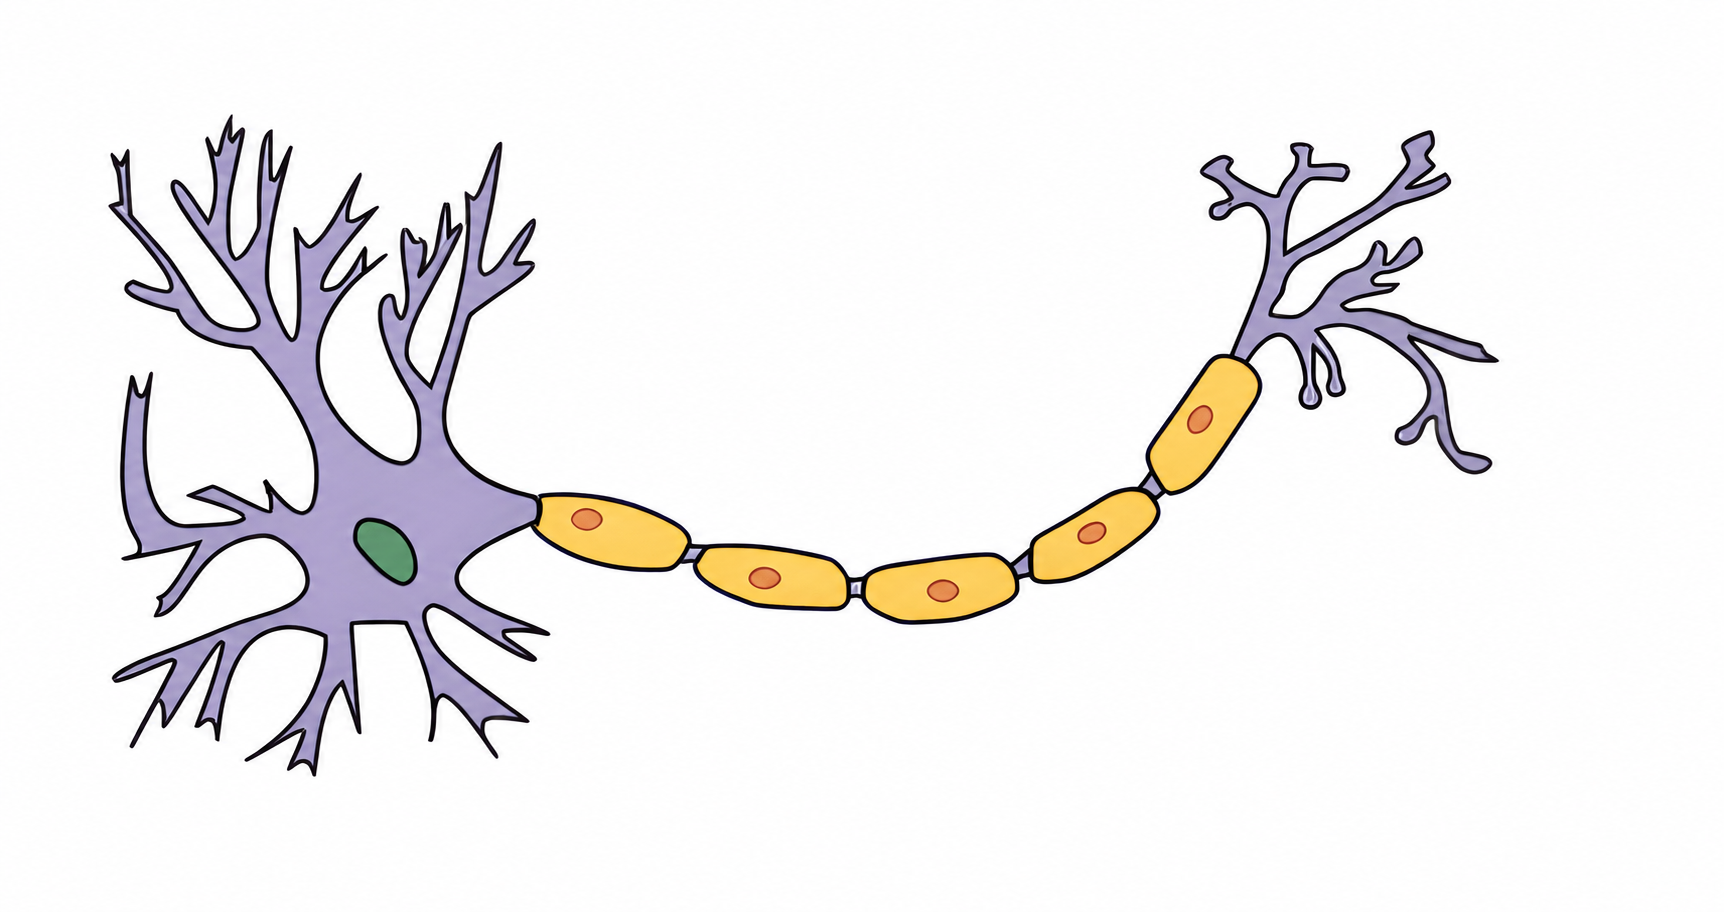
\includegraphics[width=12cm]{images/neuron.png}};

    % Dendrity
    \node (dentrites) at (-3,-3) {Dendrity};
    \draw[arr] (dentrites) -- (-3.5,-2);
    \draw[arr] (dentrites) -- (-2.7,-2);

    % Cell body
    \node (cellbody) at (-1.2,0.8) {Tělo buňky};
    \draw[arr] (cellbody) -- (-3,-0.3);

    % Axon trunk
    \node (cellbody) at (1,-2.5) {Axonové vlákno};
    \draw[arr] (cellbody) -- (0.7,-1.2);

    % Synapses
    \node (synapses) at (4.5,3) {Synapse};
    \draw[arr] (synapses) -- (3.2,2.1);
    \draw[arr] (synapses) -- (4,1);

\end{tikzpicture}
